\documentclass[aspectratio=169]{beamer}

% Default packages
\usepackage[T1]{fontenc}
\usepackage[english]{babel}
\usepackage{pgfplots}
\pgfplotsset{compat=newest}
\usepackage{booktabs}
\usepackage{siunitx}
\usepackage{amsmath}

% Font selection
% Latin Modern
\usepackage{lmodern}
% Verdana font type
%\usepackage{verdana}
% Helvetica
%\usepackage{helvet}
% Times (text and math)
%\usepackage{newtx, newtxmath}
% Nice font combination
%\usepackage{mathptmx} % math
%\usepackage{sourcesanspro} % sans-serif
\usepackage{charter} % serif

%Avoid shaded in RMarkdown



% Use DTU theme, see below for options
\usetheme[department=compute]{DTU}

\title[Automated and Early Detection of Disease Outbreaks]{Automated and
Early Detection of Disease Outbreaks}
\author{Kasper Schou Telkamp}
\institute{Section for Dynamical Systems}
\date{2023-02-09}
	
\newcommand{\tabitem}{{\color{dtured}$\bullet$} }

\DeclareMathOperator{\E}{E}
\DeclareMathOperator{\V}{V}
\DeclareMathOperator{\G}{G}
\DeclareMathOperator{\N}{N}
\DeclareMathOperator{\NB}{NB}
\DeclareMathOperator{\Pois}{Pois}
\DeclareMathOperator{\Geom}{Geom}


\begin{document}


\frame{
	\maketitle
}

\frame{
	\frametitle{Outline}
	\tableofcontents
}

\hypertarget{data-exploration}{%
\section{Data exploration}\label{data-exploration}}

\hypertarget{vtec-stec}{%
\subsection*{VTEC / STEC}\label{vtec-stec}}

\begin{frame}{VTEC / STEC}
\tiny

\begin{table}
\centering\begingroup\fontsize{12}{14}\selectfont

\begin{tabular}{llll}
\toprule
Date & ageGroup & $y_{it}$ & $x_{it}$\\
\midrule
2008-01-01 & <1 year & 2 & 64137\\
2008-01-01 & 1-4 years & 2 & 259910\\
2008-01-01 & 5-14 years & 2 & 680529\\
2008-01-01 & 15-24 years & 1 & 635838\\
... & ... & ... & ...\\
2022-12-01 & 5-14 years & 5 & 634139\\
2022-12-01 & 15-24 years & 1 & 721286\\
2022-12-01 & 25-64 years & 10 & 3031374\\
2022-12-01 & 65+ years & 12 & 1204892\\
\bottomrule
\end{tabular}
\endgroup{}
\end{table}

\normalsize
\end{frame}

\begin{frame}{VTEC / STEC}
\protect\hypertarget{vtec-stec-1}{}
\tiny

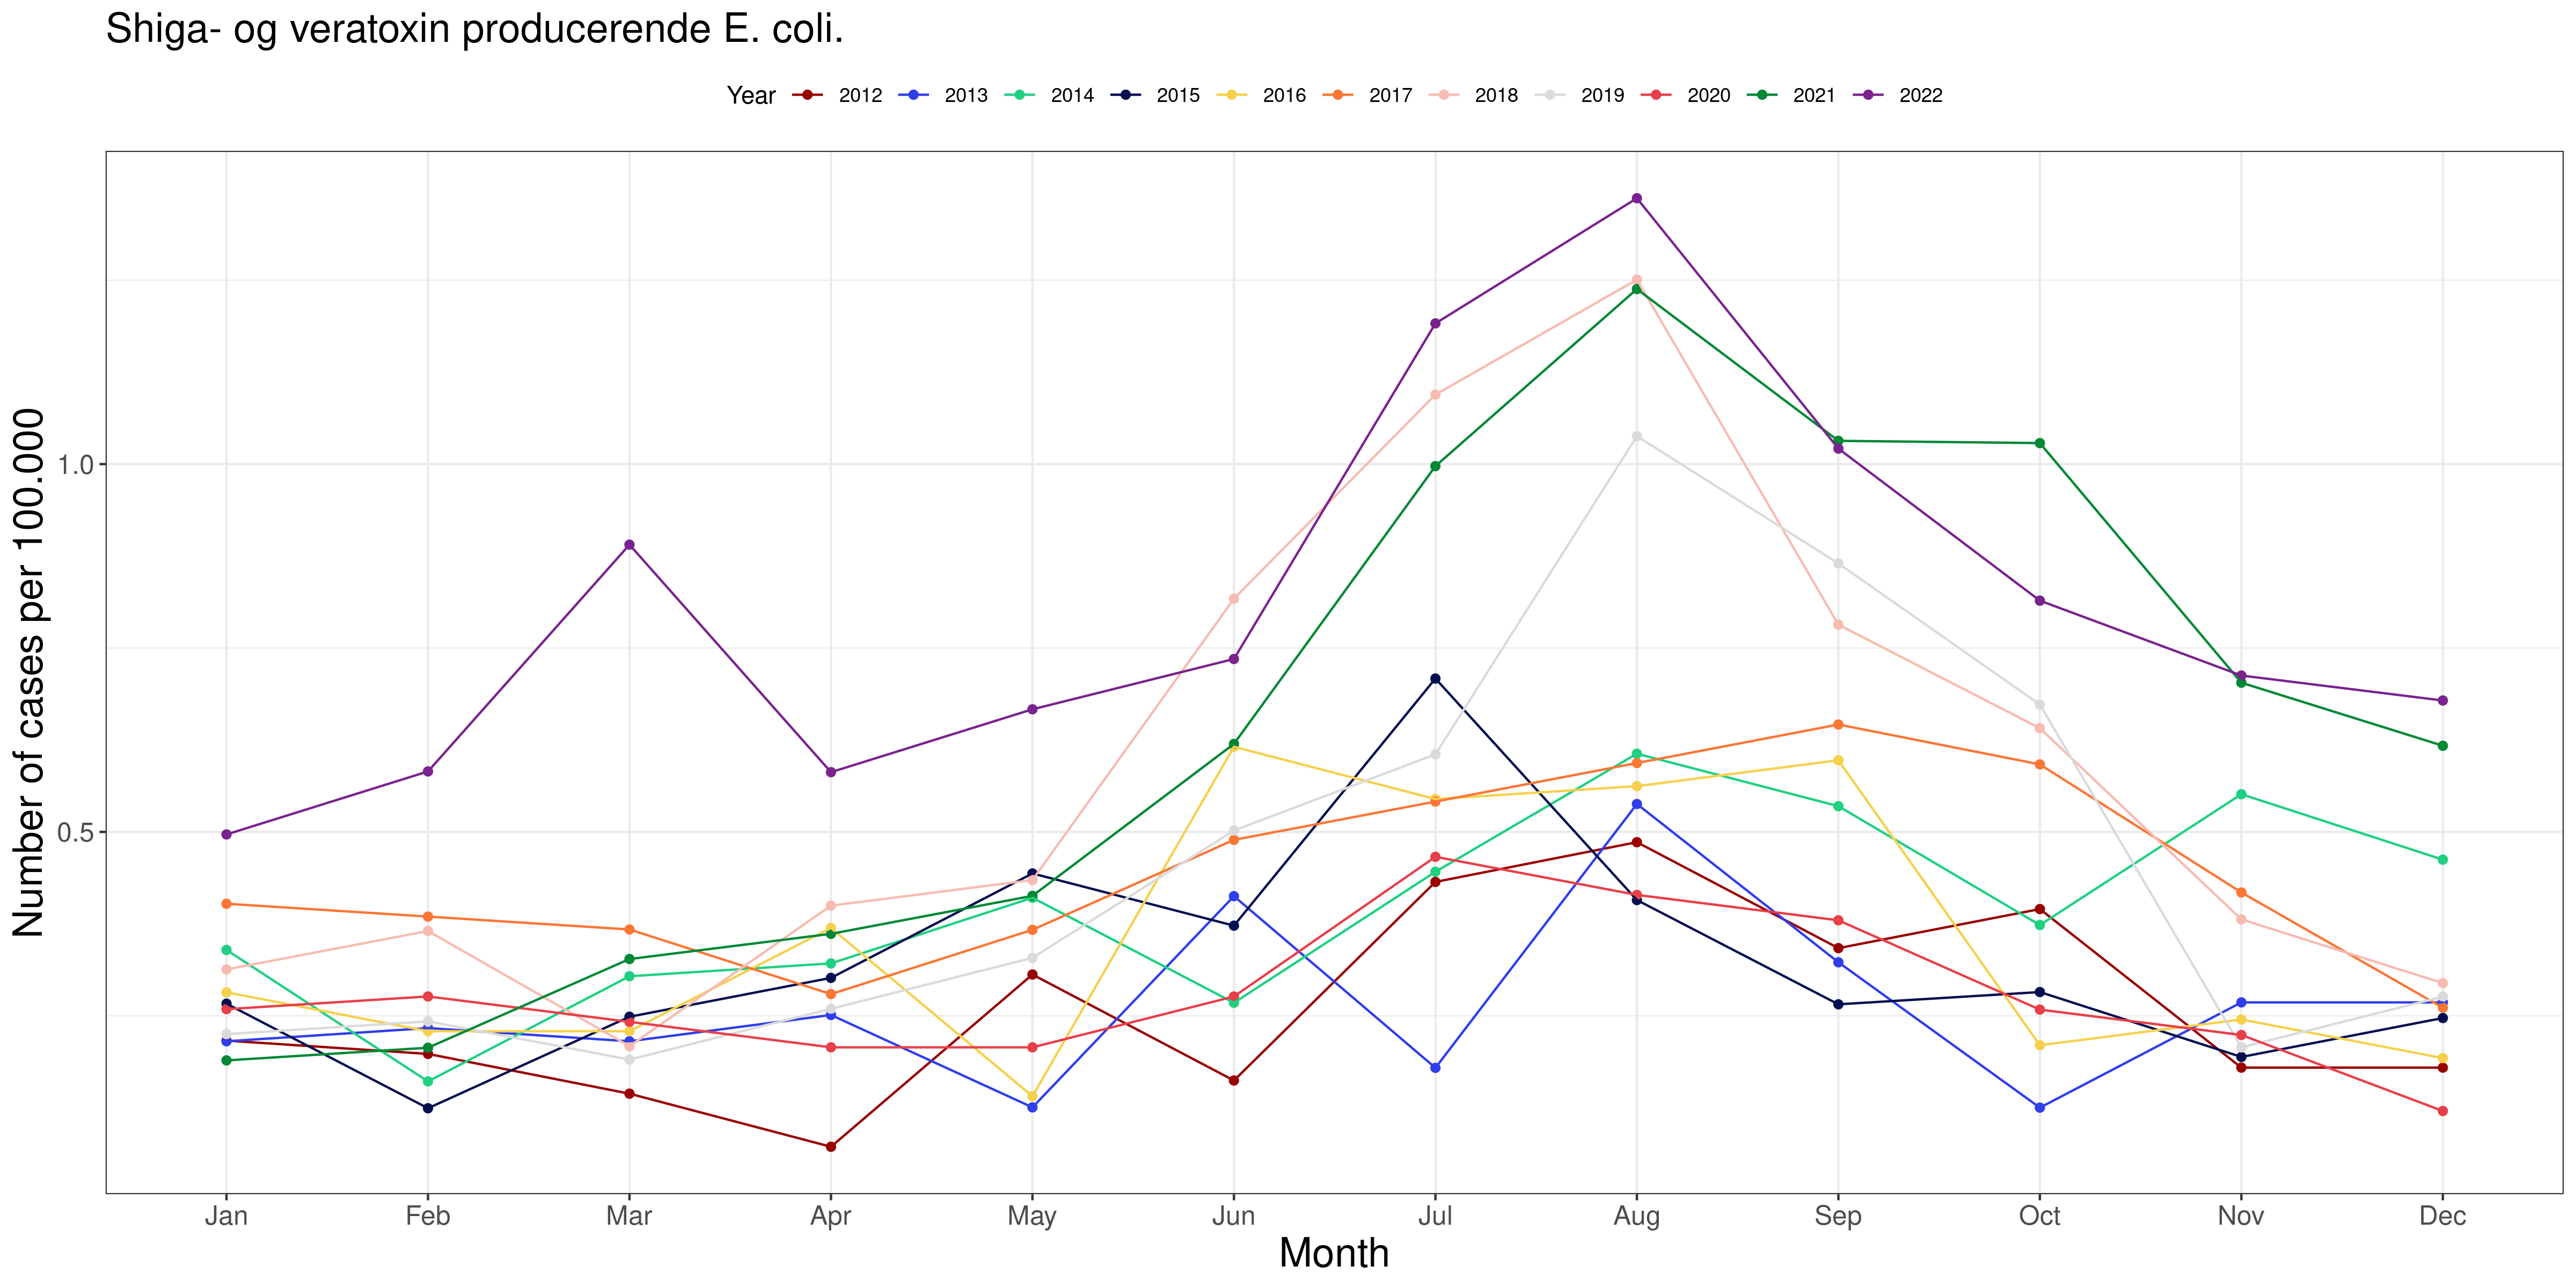
\includegraphics[width=1\linewidth]{../figures/EpixSTEC}

\normalsize
\end{frame}

\begin{frame}{VTEC / STEC}
\protect\hypertarget{vtec-stec-2}{}
\tiny

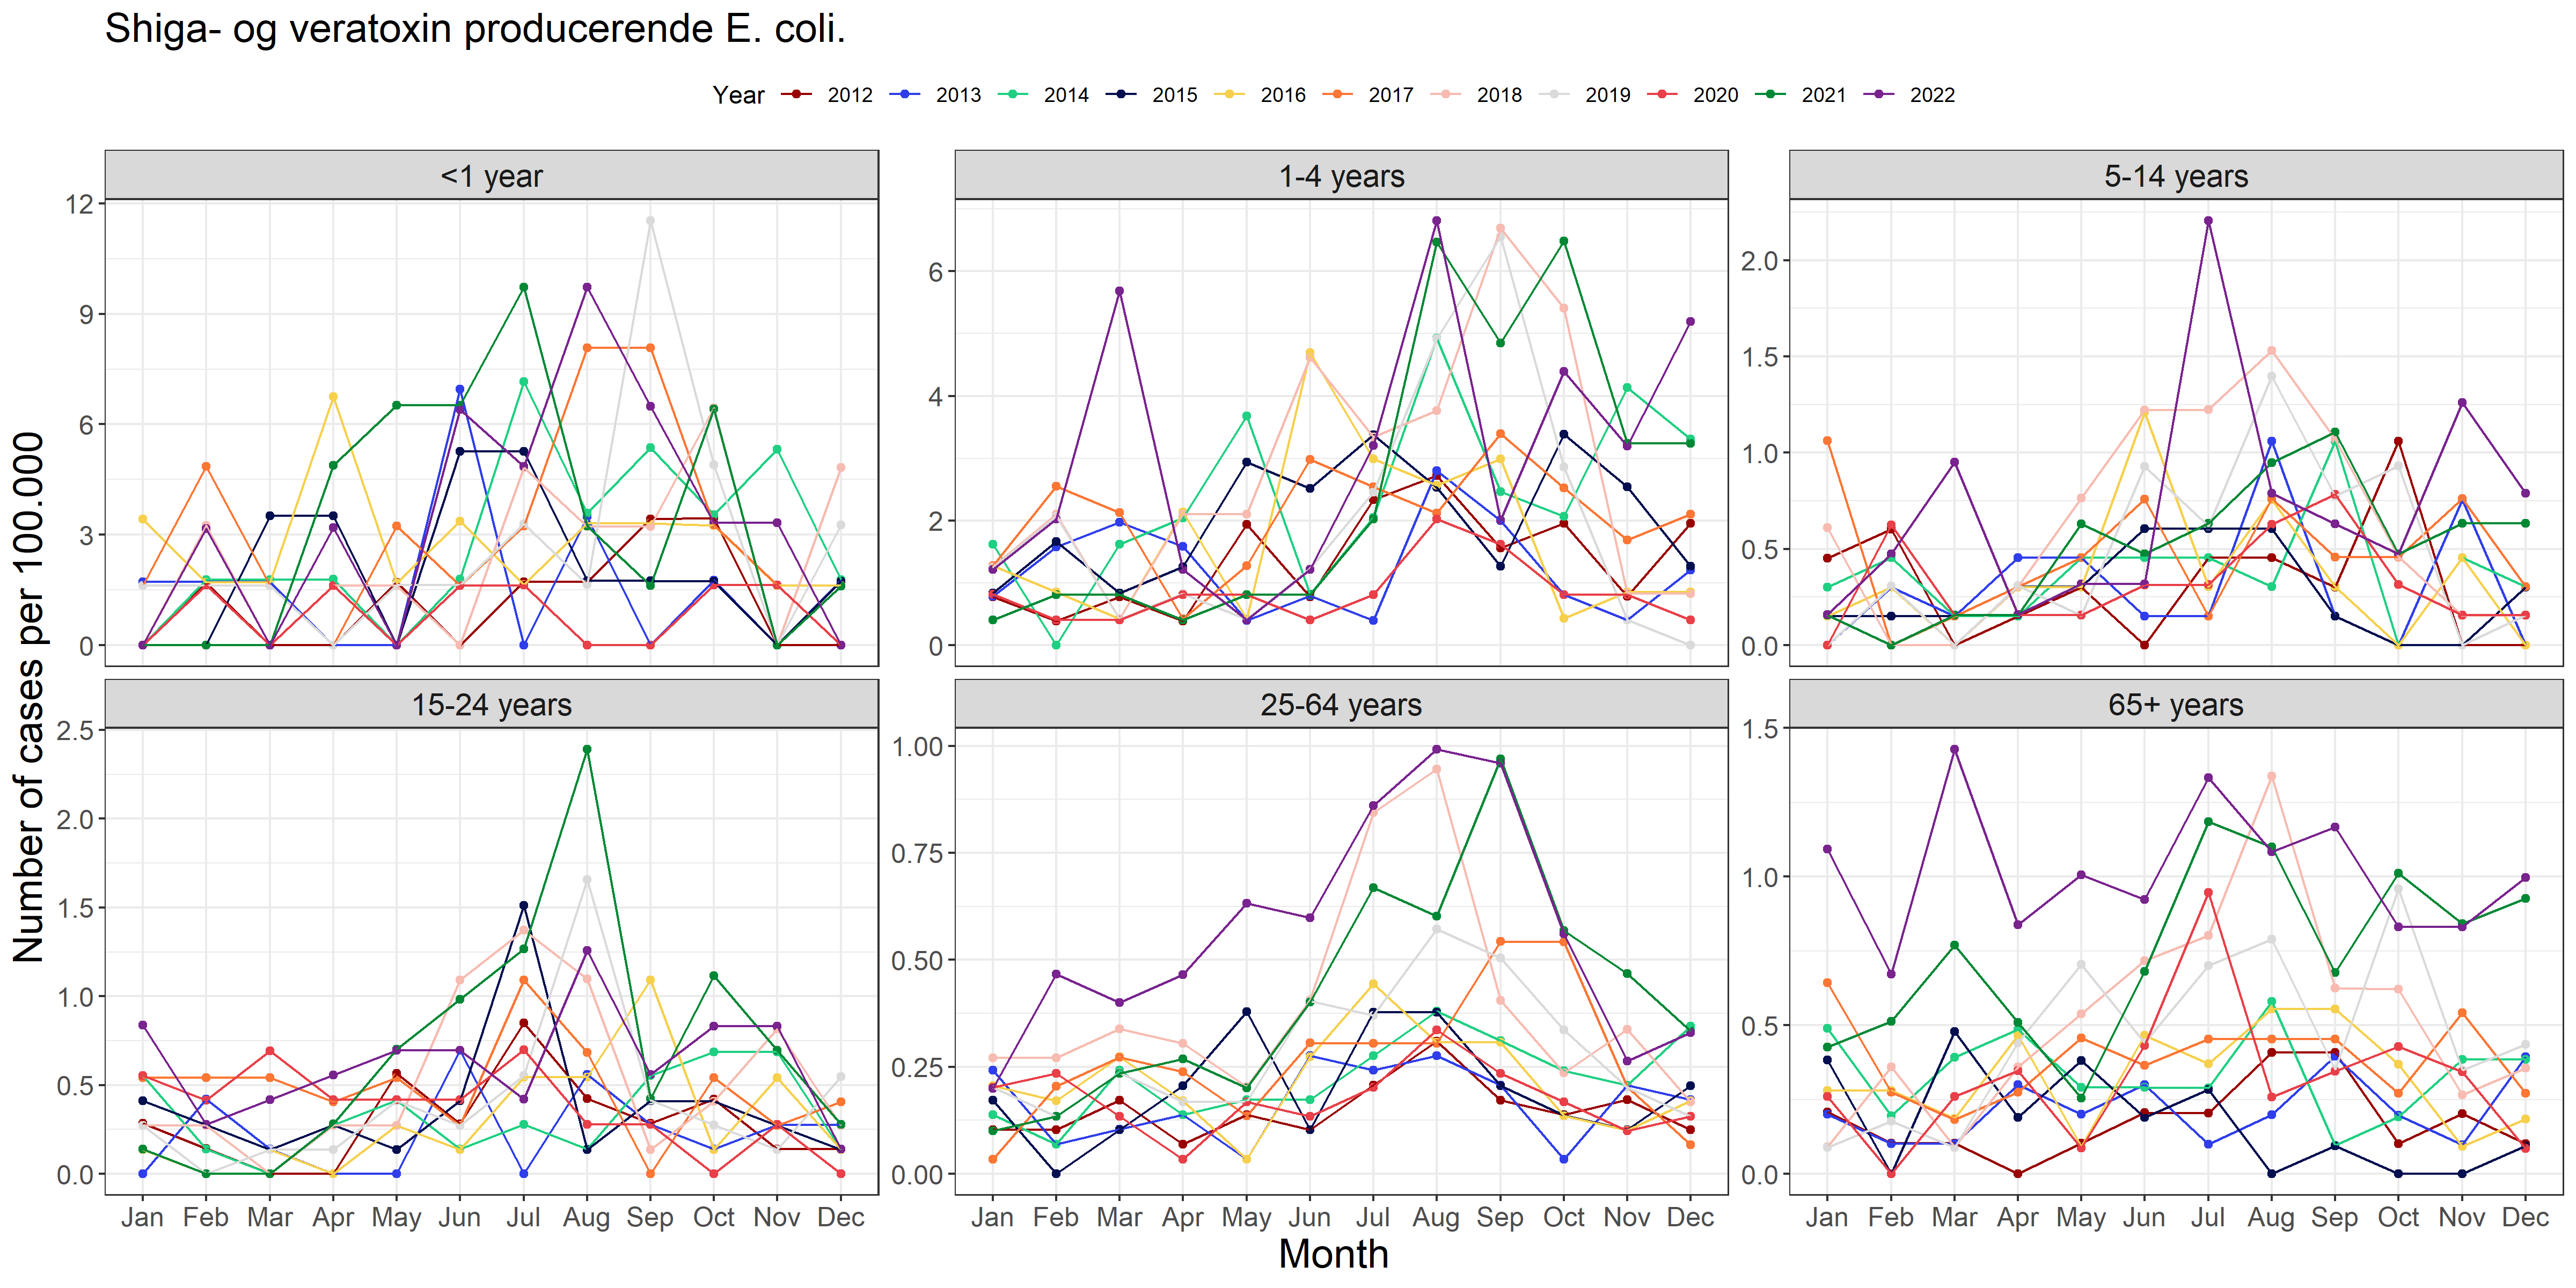
\includegraphics[width=1\linewidth]{../figures/STECxEpixAgeGroup}

\normalsize
\end{frame}

\begin{frame}{VTEC / STEC}
\protect\hypertarget{vtec-stec-3}{}
\tiny

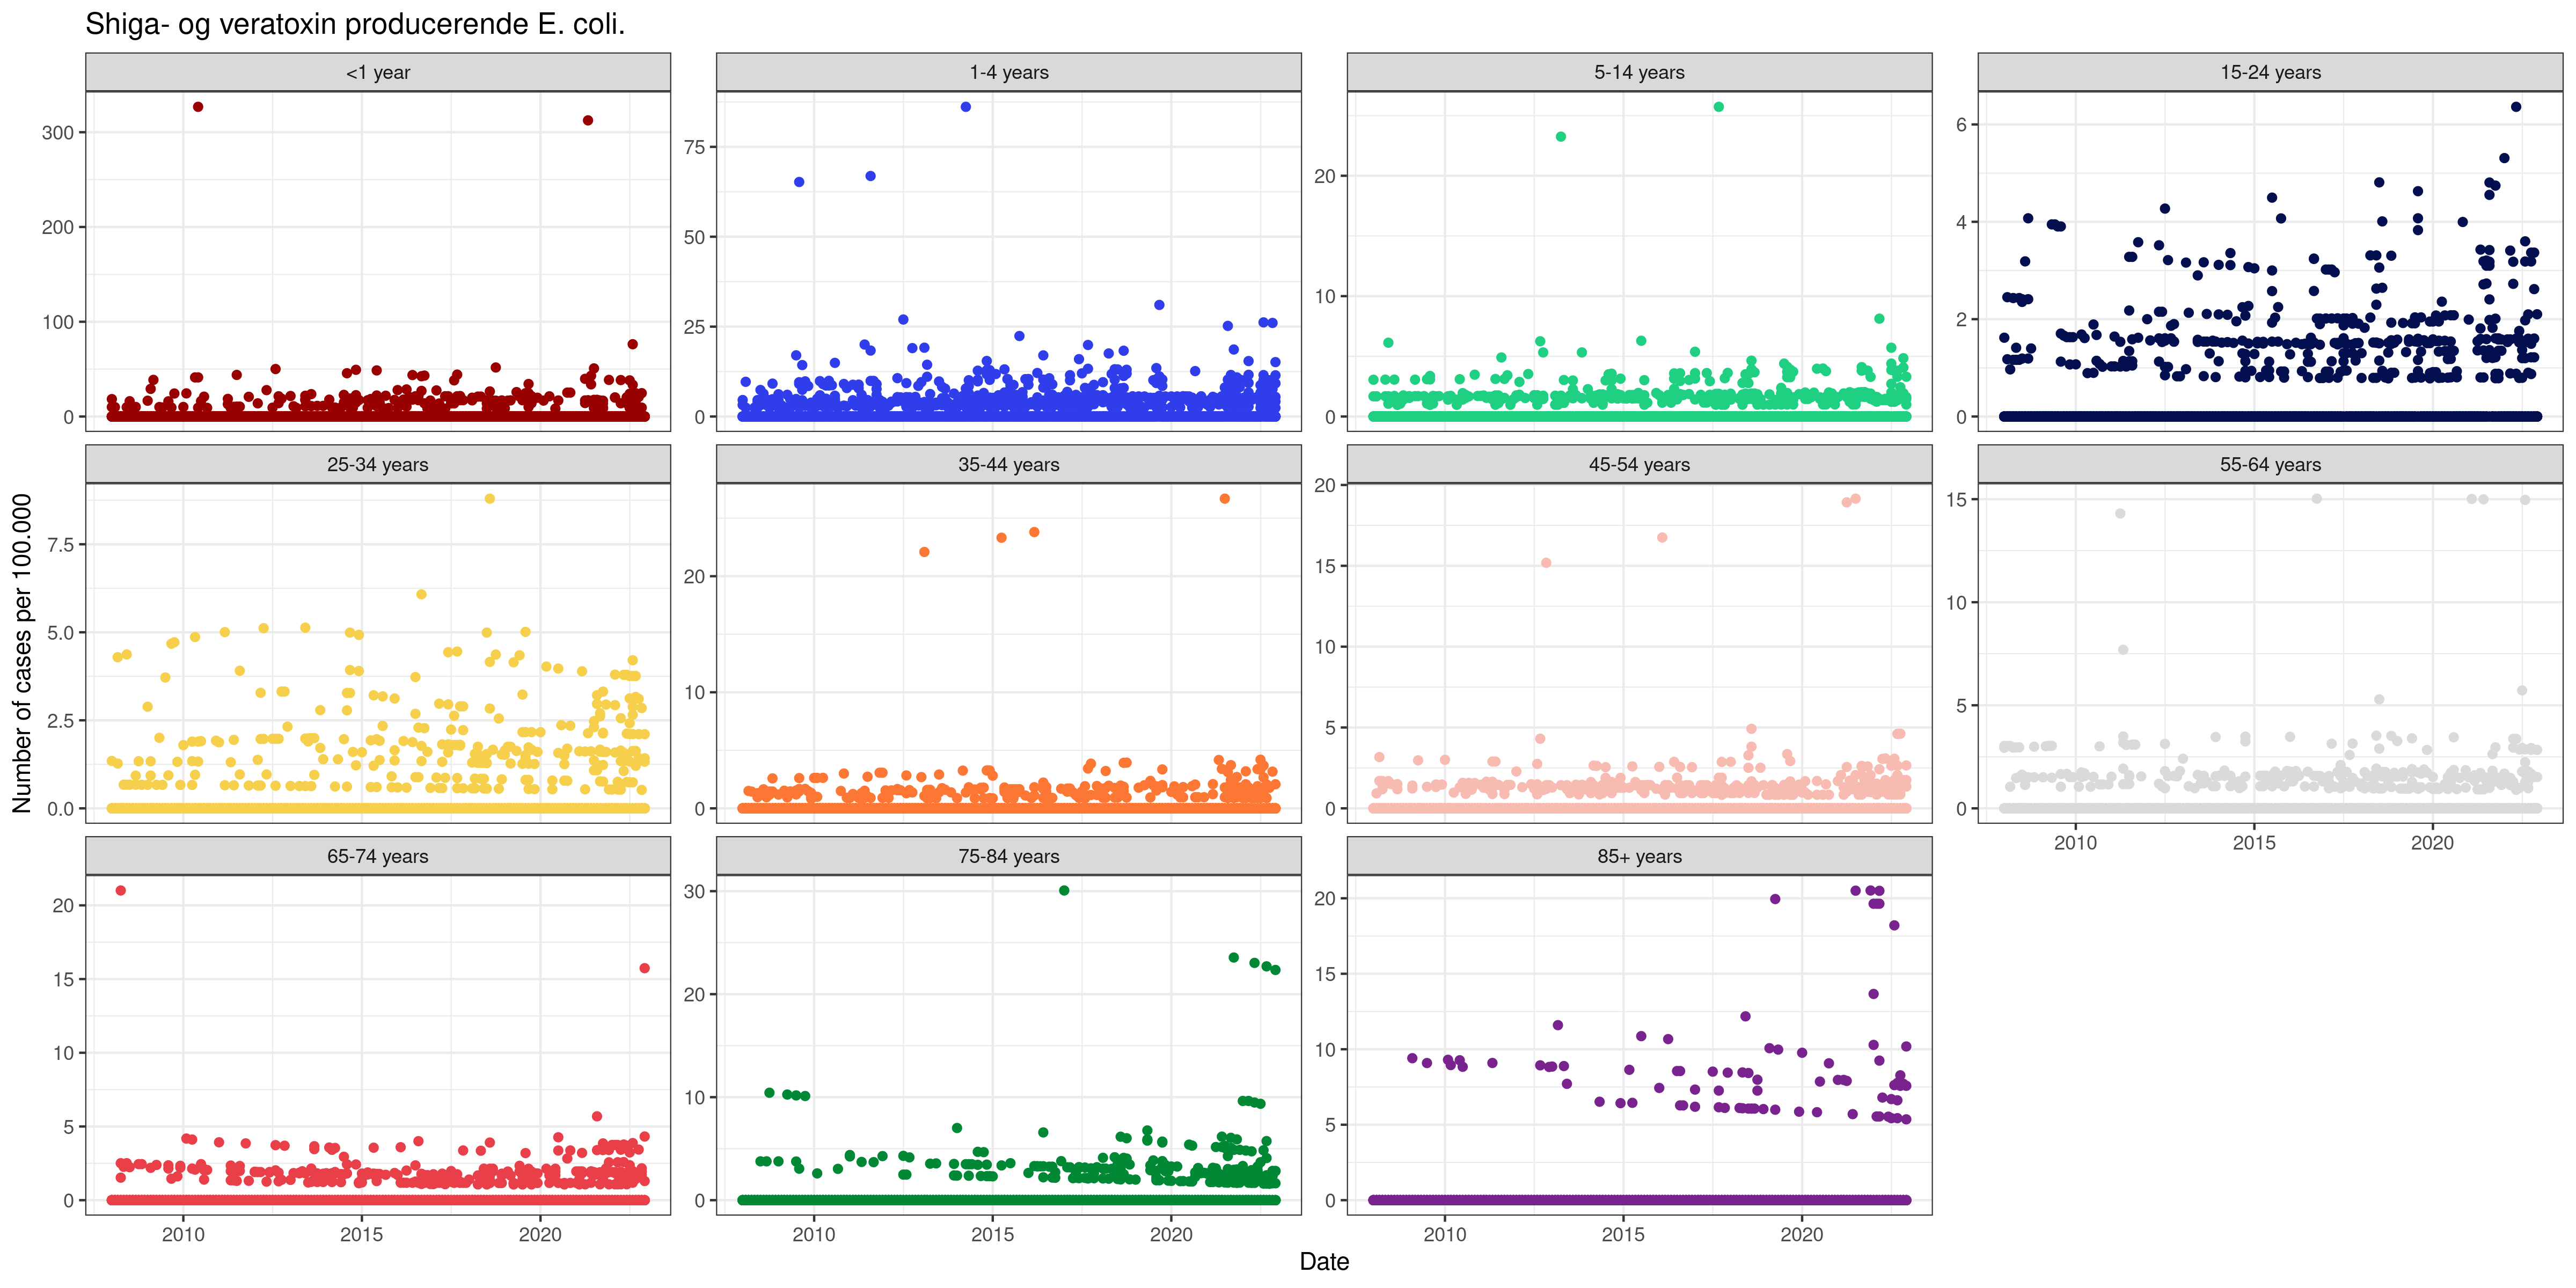
\includegraphics[width=1\linewidth]{../figures/ShigaogveratoxinproducerendeEcolixAgeGroup}

\normalsize
\end{frame}

\hypertarget{hierachical-poisson-normal-model}{%
\section{Hierachical Poisson-Normal
model}\label{hierachical-poisson-normal-model}}

\hypertarget{formulation}{%
\subsection{Formulation}\label{formulation}}

\begin{frame}{Formulation}
The conditional distribution, \(Y|u\), of the count observations are
assumed to be a Poisson distribution with intensities \(\lambda_{it}\).
Also, we shall assume that the count is proportional to the population
size, \(x_{it}\), within each age group, \(i\), at a given time point,
\(t\). Hence, in terms of the canonical link for the Poisson
distribution the model for the fixed effect is

\begin{equation}
  \log(\lambda_{it})=\mathbf{X}_i^T\mathbf{\beta}_{it}+\log(x_{it})
\end{equation}

Here \(\mathbf{X}_i\) is \(T\times6\)-dimensional, and
\(\mathbf{\beta}_{it}\) contains the corresponding fixed effect
parameter. The random effects \(u_{it}\) are assumed to be Gaussian.

\begin{equation}
  u_{it} = \epsilon_{it}
\end{equation}

where \(\epsilon_{it}\sim\N(0,\sigma^2)\) is a white noise process, and
\(\sigma\) is a model parameter.
\end{frame}

\begin{frame}{Fomulation}
\protect\hypertarget{fomulation}{}
Henceforth, the model can be formulated as a two-level hierarchical
model

\begin{subequations}
  \begin{alignat}{2}
    Y_{it}|u_{it} &\sim \Pois (\lambda_{it}e^{u_{it}}) \label{eq:pois_ln0} \\ 
    u_{it} &\sim \N(0,\sigma^2) \label{eq:pois_ln1}
  \end{alignat}
\end{subequations}
\end{frame}

\hypertarget{results}{%
\subsection{Results}\label{results}}

\begin{frame}{Results}
\tiny

\begin{table}
\centering\begingroup\fontsize{10}{12}\selectfont

\begin{tabular}{lrr}
\toprule
Parameter & Estimate & Std. Error\\
\midrule
$\beta_{<1 year}$ & 10.83 & 0.11\\
$\beta_{1-4 years}$ & 13.64 & 0.09\\
$\beta_{5-14 years}$ & 13.94 & 0.10\\
$\beta_{15-24 years}$ & 14.05 & 0.09\\
$\beta_{25-64 years}$ & 16.61 & 0.08\\
$\beta_{65+ years}$ & 14.83 & 0.09\\
$\sigma$ & 1.01 & 0.04\\
\bottomrule
\end{tabular}
\endgroup{}
\end{table}

\normalsize
\end{frame}

\begin{frame}{Results}
\protect\hypertarget{results-1}{}
\tiny

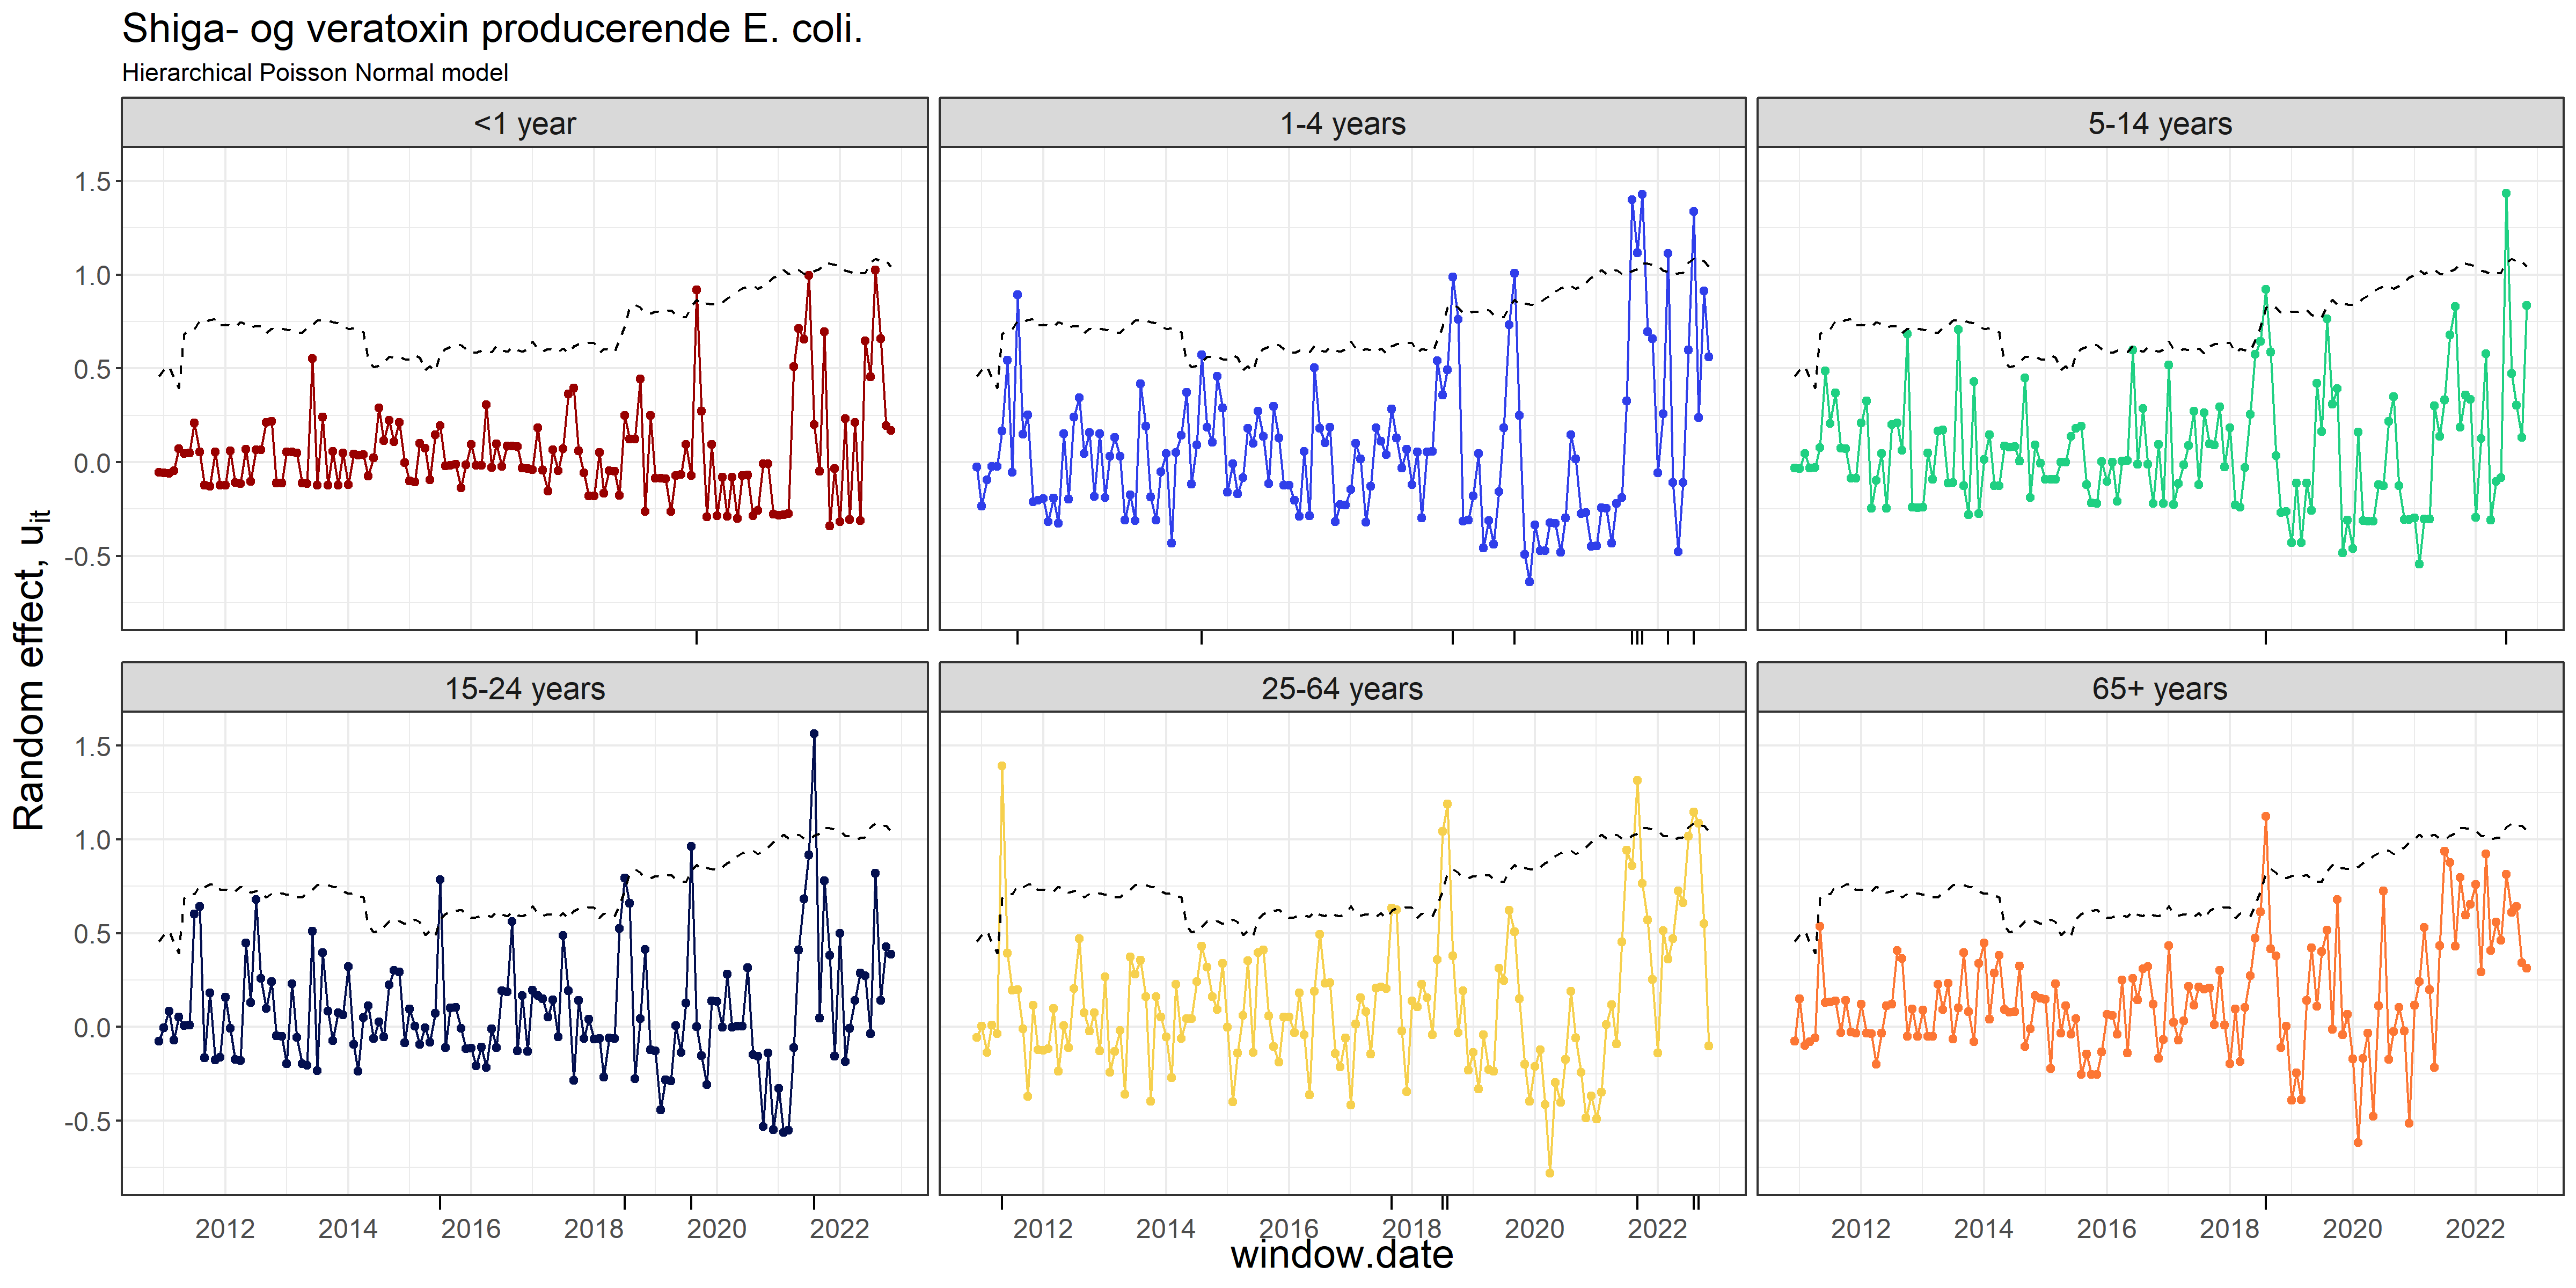
\includegraphics[width=1\linewidth]{../figures/windowedSTEDPoisN}

\normalsize
\end{frame}

\begin{frame}{Results}
\protect\hypertarget{results-2}{}
\tiny

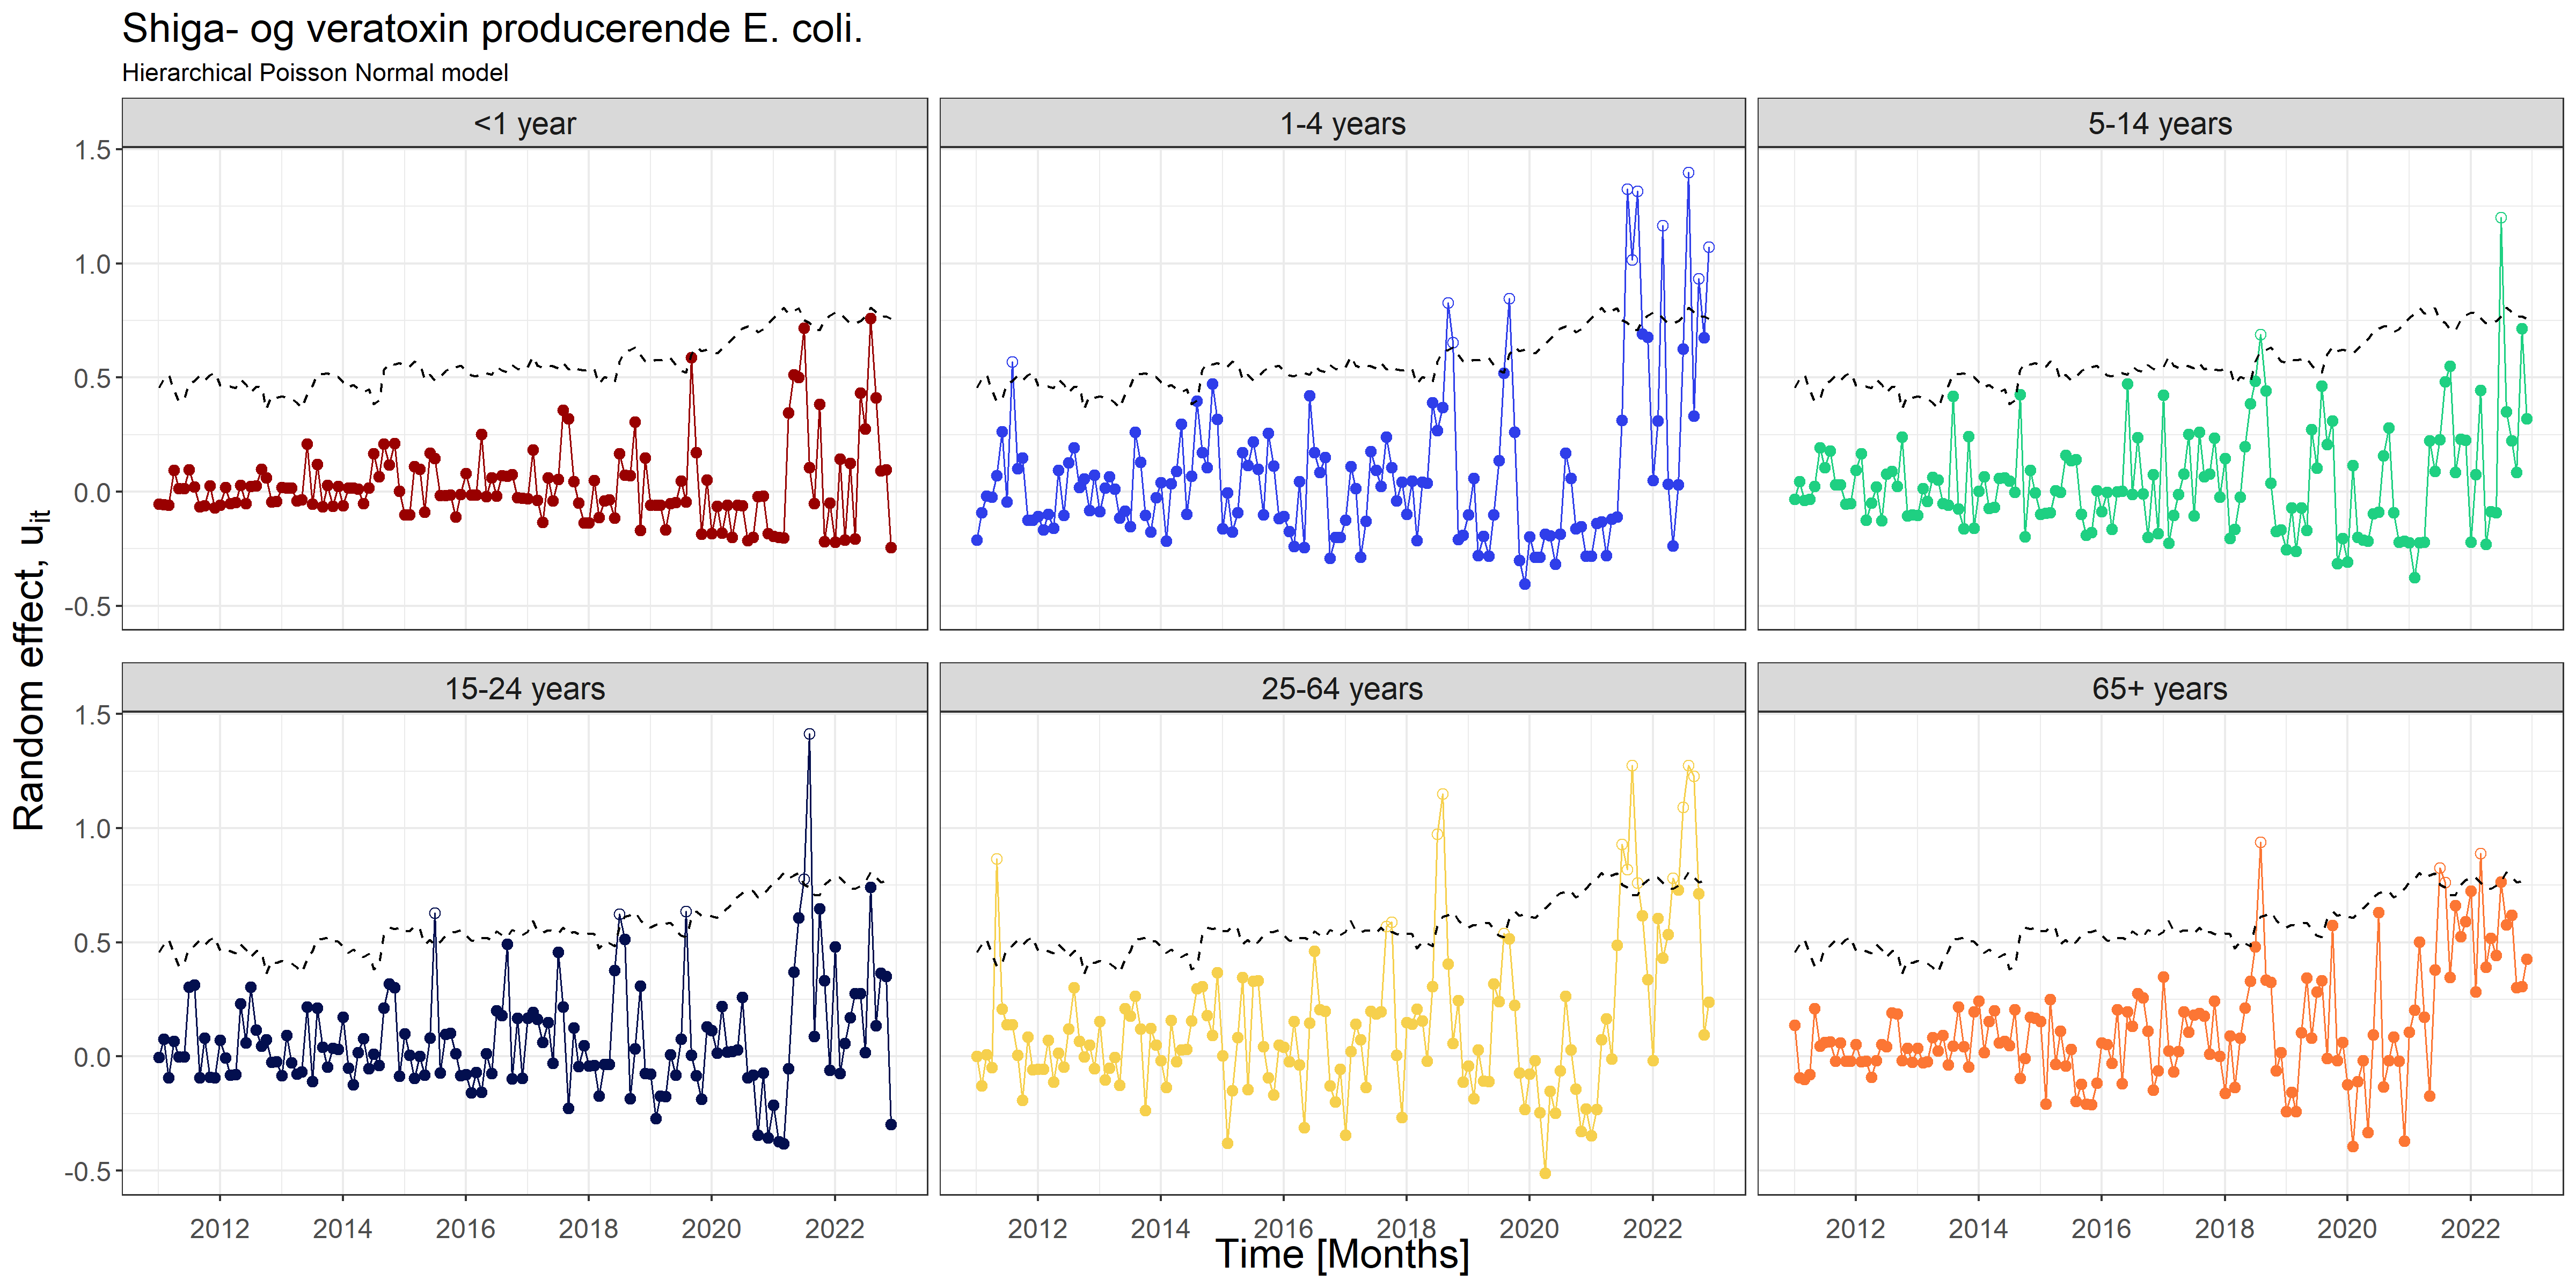
\includegraphics[width=1\linewidth]{../figures/windowedSTEDPoisNExclude}

\normalsize
\end{frame}

\hypertarget{hierachical-poisson-gamma-model}{%
\section{Hierachical Poisson-Gamma
model}\label{hierachical-poisson-gamma-model}}

\hypertarget{formulation-1}{%
\subsection{Formulation}\label{formulation-1}}

\begin{frame}{Formulation}
Likewise, in the compound Poisson-Gamma model the conditional
distribution, \(Y|u\), of the count observations are assumed to be a
Poisson distribution, but this time the intensities, \(\lambda_{it}\),
are defined as

\begin{equation}
  \log(\lambda_{it})=\mathbf{X}_i^T\mathbf{\beta}_{it}+\log(x_{it})
\end{equation}

Here \(\mathbf{X}_i\) is \(T\times6\)-dimensional, and
\(\mathbf{\beta}_{it}\) contains the corresponding fixed effect
parameter. Additionally, the random effects \(u_{it}\) are assumed to be
Gamma distributed.
\end{frame}

\begin{frame}{Formulation}
\protect\hypertarget{formulation-2}{}
Subsequently, the model can be formulated as a two-level hierarchical
model

\begin{subequations} \label{eq:PoisGam}
  \begin{alignat}{2}
    Y_{it}|u_{it} &\sim \Pois (\lambda_{it}u_{it}) \label{eq:pois_g0} \\ 
    u_{it} &\sim \G(1/\phi_{i},\phi_{i}) \label{eq:pois_g1}
  \end{alignat}
\end{subequations}
\end{frame}

\hypertarget{probability-function-for-y}{%
\subsection{\texorpdfstring{Probability function for
\(Y\)}{Probability function for Y}}\label{probability-function-for-y}}

\begin{frame}{Probability function for \(Y\)}
\begin{equation} \label{eq:pdfMix}
  \begin{aligned}
    P[Y=y_i]&=g_{Y}(y;\lambda, \phi) \\
    &=\frac{\lambda^{y}}{y!\Gamma(1/\phi)\phi^{1/\phi}}\frac{\phi^{y+1/\phi}\Gamma(y+1/\phi)}{(\lambda \phi + 1)^{y+1/\phi}} \\
    &=\frac{\Gamma(y+1/\phi)}{\Gamma(1/\phi)y!}\frac{1}{(\lambda\phi+1)^{1/\phi}}\bigg(\frac{\lambda\phi}{\lambda\phi+1}\bigg)^{y} \\
    &=\begin{pmatrix} y+1/\phi-1 \\ y \end{pmatrix} \frac{1}{(\lambda\phi+1)^{1/\phi}}\bigg(\frac{\lambda\phi}{\lambda\phi+1}\bigg)^{y} \ , \ for \ y = 0, 1, 2, \dots
  \end{aligned}
\end{equation}

where we have used the convention

\begin{equation}
  \begin{pmatrix} z\\y \end{pmatrix} = \frac{\Gamma(z+1)}{\Gamma(z+1-y)y!}
\end{equation}

The marginal distribution of \(Y\) is a negative binomial distribution,
\(Y\sim \NB\big(1/\phi,1/(\lambda \phi+1)\big)\)
\end{frame}

\begin{frame}{Proof}
\protect\hypertarget{proof}{}
The probability function for the conditional distribution of \(Y\) for
given \(u\)

\begin{equation} \label{eq:pdfPois}
  f_{Y|u}(y;\lambda, u)=\frac{(\lambda u)^y}{y!} \exp (-\lambda u)
\end{equation}

and the probability density function for the distribution of \(u\) is

\begin{equation} \label{eq:pdfGamma}
  f_{u}(u;\phi)=\frac{1}{\phi \Gamma(1/\phi)} \bigg(\frac{u}{\phi}\bigg)^{1/\phi-1} \exp (-u/\phi)
\end{equation}
\end{frame}

\begin{frame}{Proof}
\protect\hypertarget{proof-1}{}
Given \eqref{eq:pdfPois} and \eqref{eq:pdfGamma}, the probability
function for the marginal distribution of \(Y\) is determined from

\begin{equation} \label{eq:marMix}
  \begin{aligned}
    g_{Y}(y;\lambda,\phi)&=\int_{u=0}^\infty f_{Y|u}(y;\lambda, u) f_{u}(u;\phi) \,du \\
    &=\int_{u=0}^\infty \frac{(\lambda u)^y}{y!} \exp (-\lambda u) \frac{1}{\phi \Gamma(1/\phi)} \bigg(\frac{u}{\phi}\bigg)^{1/\phi-1} \exp (-u/\phi) \,du\\
    &=\frac{\lambda^{y}}{y!\Gamma(1/\phi)\phi^{1/\phi}} \int_{u=0}^\infty u^{y+1/\phi-1} \exp \big(-u(\lambda \phi+1)/\phi\big) \,du
  \end{aligned}
\end{equation}
\end{frame}

\begin{frame}{Proof}
\protect\hypertarget{proof-2}{}
In \eqref{eq:marMix} it is noted that the integrand is the \emph{kernel}
in the probability density function for a Gamma distribution,
\(\G\big(y+1/\phi,\phi/(\lambda \phi+1)\big)\). As the integral of the
density shall equal one, we find by adjusting the norming constant that

\begin{equation}
  \int_{u=0}^\infty u^{y+1/\phi-1} \exp \bigg(-u/\Big(\phi/(\lambda \phi+1)\Big)\bigg) \,du = \frac{\phi^{y+1/\phi}\Gamma(y+1/\phi)}{(\lambda \phi + 1)^{y+1/\phi}}
\end{equation}

and then \eqref{eq:pdfMix} follows
\end{frame}

\hypertarget{inference-on-individual-group-means}{%
\subsection{Inference on individual group
means}\label{inference-on-individual-group-means}}

\begin{frame}{Inference on individual group means}
Consider the hierarchical Poisson-Gamma model in \eqref{eq:PoisGam}, and
assume that a value \(Y=y\) has been observed. Then the conditional
distribution of \(u\) for given \(Y=y\) is a Gamma distribution,

\begin{equation}
  u|Y=y\sim \G\big(y+1/\phi,\phi/(\lambda \phi+1)\big)
\end{equation}

with mean

\begin{equation}
  \E[u|Y=y]=\frac{y\phi+1}{\lambda\phi+1}
\end{equation}

and variance

\begin{equation}
  \V[u|Y=y]=\frac{(y \phi^2+\phi)}{(\lambda \phi + 1)^2}
\end{equation}
\end{frame}

\begin{frame}{Proof}
\protect\hypertarget{proof-3}{}
The conditional distribution is found using Bayes Theorem

\begin{equation}
  \begin{aligned}
    g_{u}(u|Y=y)&=\frac{f_{y,u}(y,u)}{g_Y(y;\lambda, \phi)} \\
    &=\frac{f_{y|u}(y;u)g_{u}(u)}{g_{Y}(y;\lambda,\phi)} \\
    &=\frac{1}{g_{Y}(y;\lambda,\phi)}\bigg(\frac{(\lambda u)^y}{y!} \exp (-\lambda u) \frac{1}{\phi \Gamma(1/\phi)} \bigg(\frac{u}{\phi}\bigg)^{1/\phi-1} \exp (-u/\phi)\bigg) \\
    &\propto u^{y+1/\phi-1} \exp \big(- u(\lambda\phi+1)/\phi\big)
  \end{aligned}
\end{equation}

We identify the \emph{kernel} of the probability density function

\begin{equation}
  u^{y+1/\phi-1} \exp (- u(\lambda\phi+1)/\phi)
\end{equation}

as the kernel of a Gamma distribution,
\(\G(y+1/\phi,\phi/(\lambda\phi+1))\)
\end{frame}

\hypertarget{results-3}{%
\subsection{Results}\label{results-3}}

\begin{frame}{Results}
\tiny

\begin{table}
\centering\begingroup\fontsize{10}{12}\selectfont

\begin{tabular}{lrr}
\toprule
Parameter & Estimate & Std. Error\\
\midrule
$\beta_{<1 year}$ & 11.23 & 0.08\\
$\beta_{1-4 years}$ & 13.94 & 0.06\\
$\beta_{5-14 years}$ & 14.30 & 0.07\\
$\beta_{15-24 years}$ & 14.42 & 0.07\\
$\beta_{25-64 years}$ & 16.87 & 0.06\\
$\beta_{65+ years}$ & 15.24 & 0.06\\
$\phi$ & 0.45 & 0.03\\
\bottomrule
\end{tabular}
\endgroup{}
\end{table}

\normalsize
\end{frame}

\begin{frame}{Results}
\protect\hypertarget{results-4}{}
\tiny

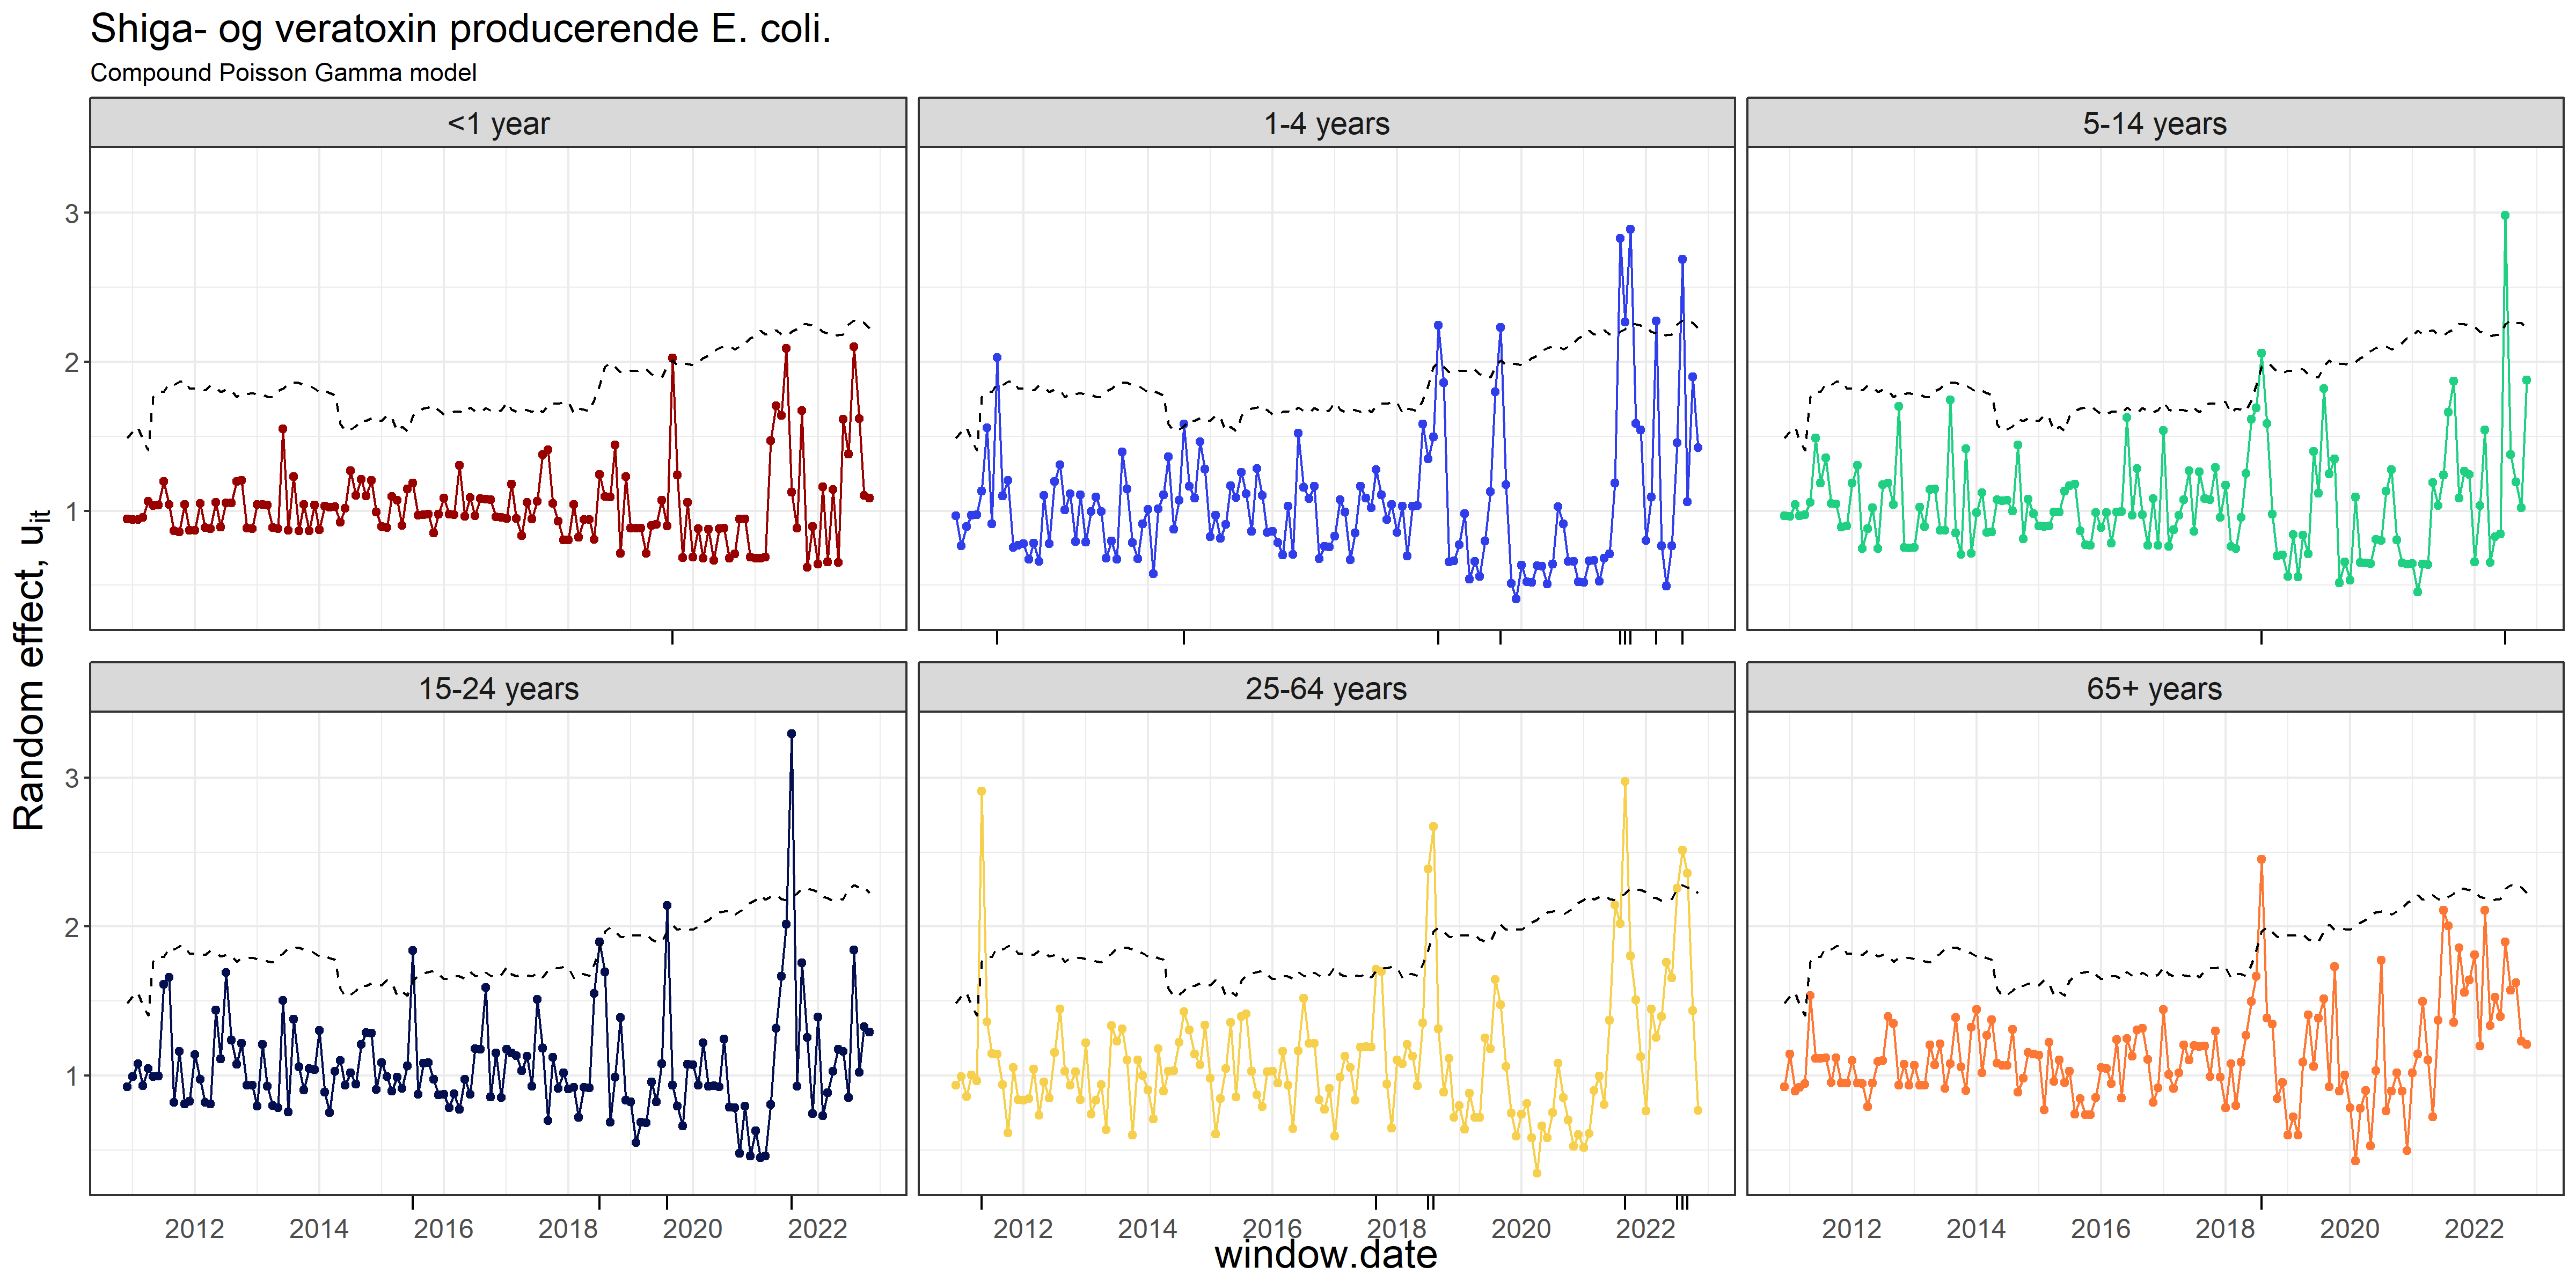
\includegraphics[width=1\linewidth]{../figures/windowedSTECPoisG}

\normalsize
\end{frame}

\begin{frame}{Results}
\protect\hypertarget{results-5}{}
\tiny

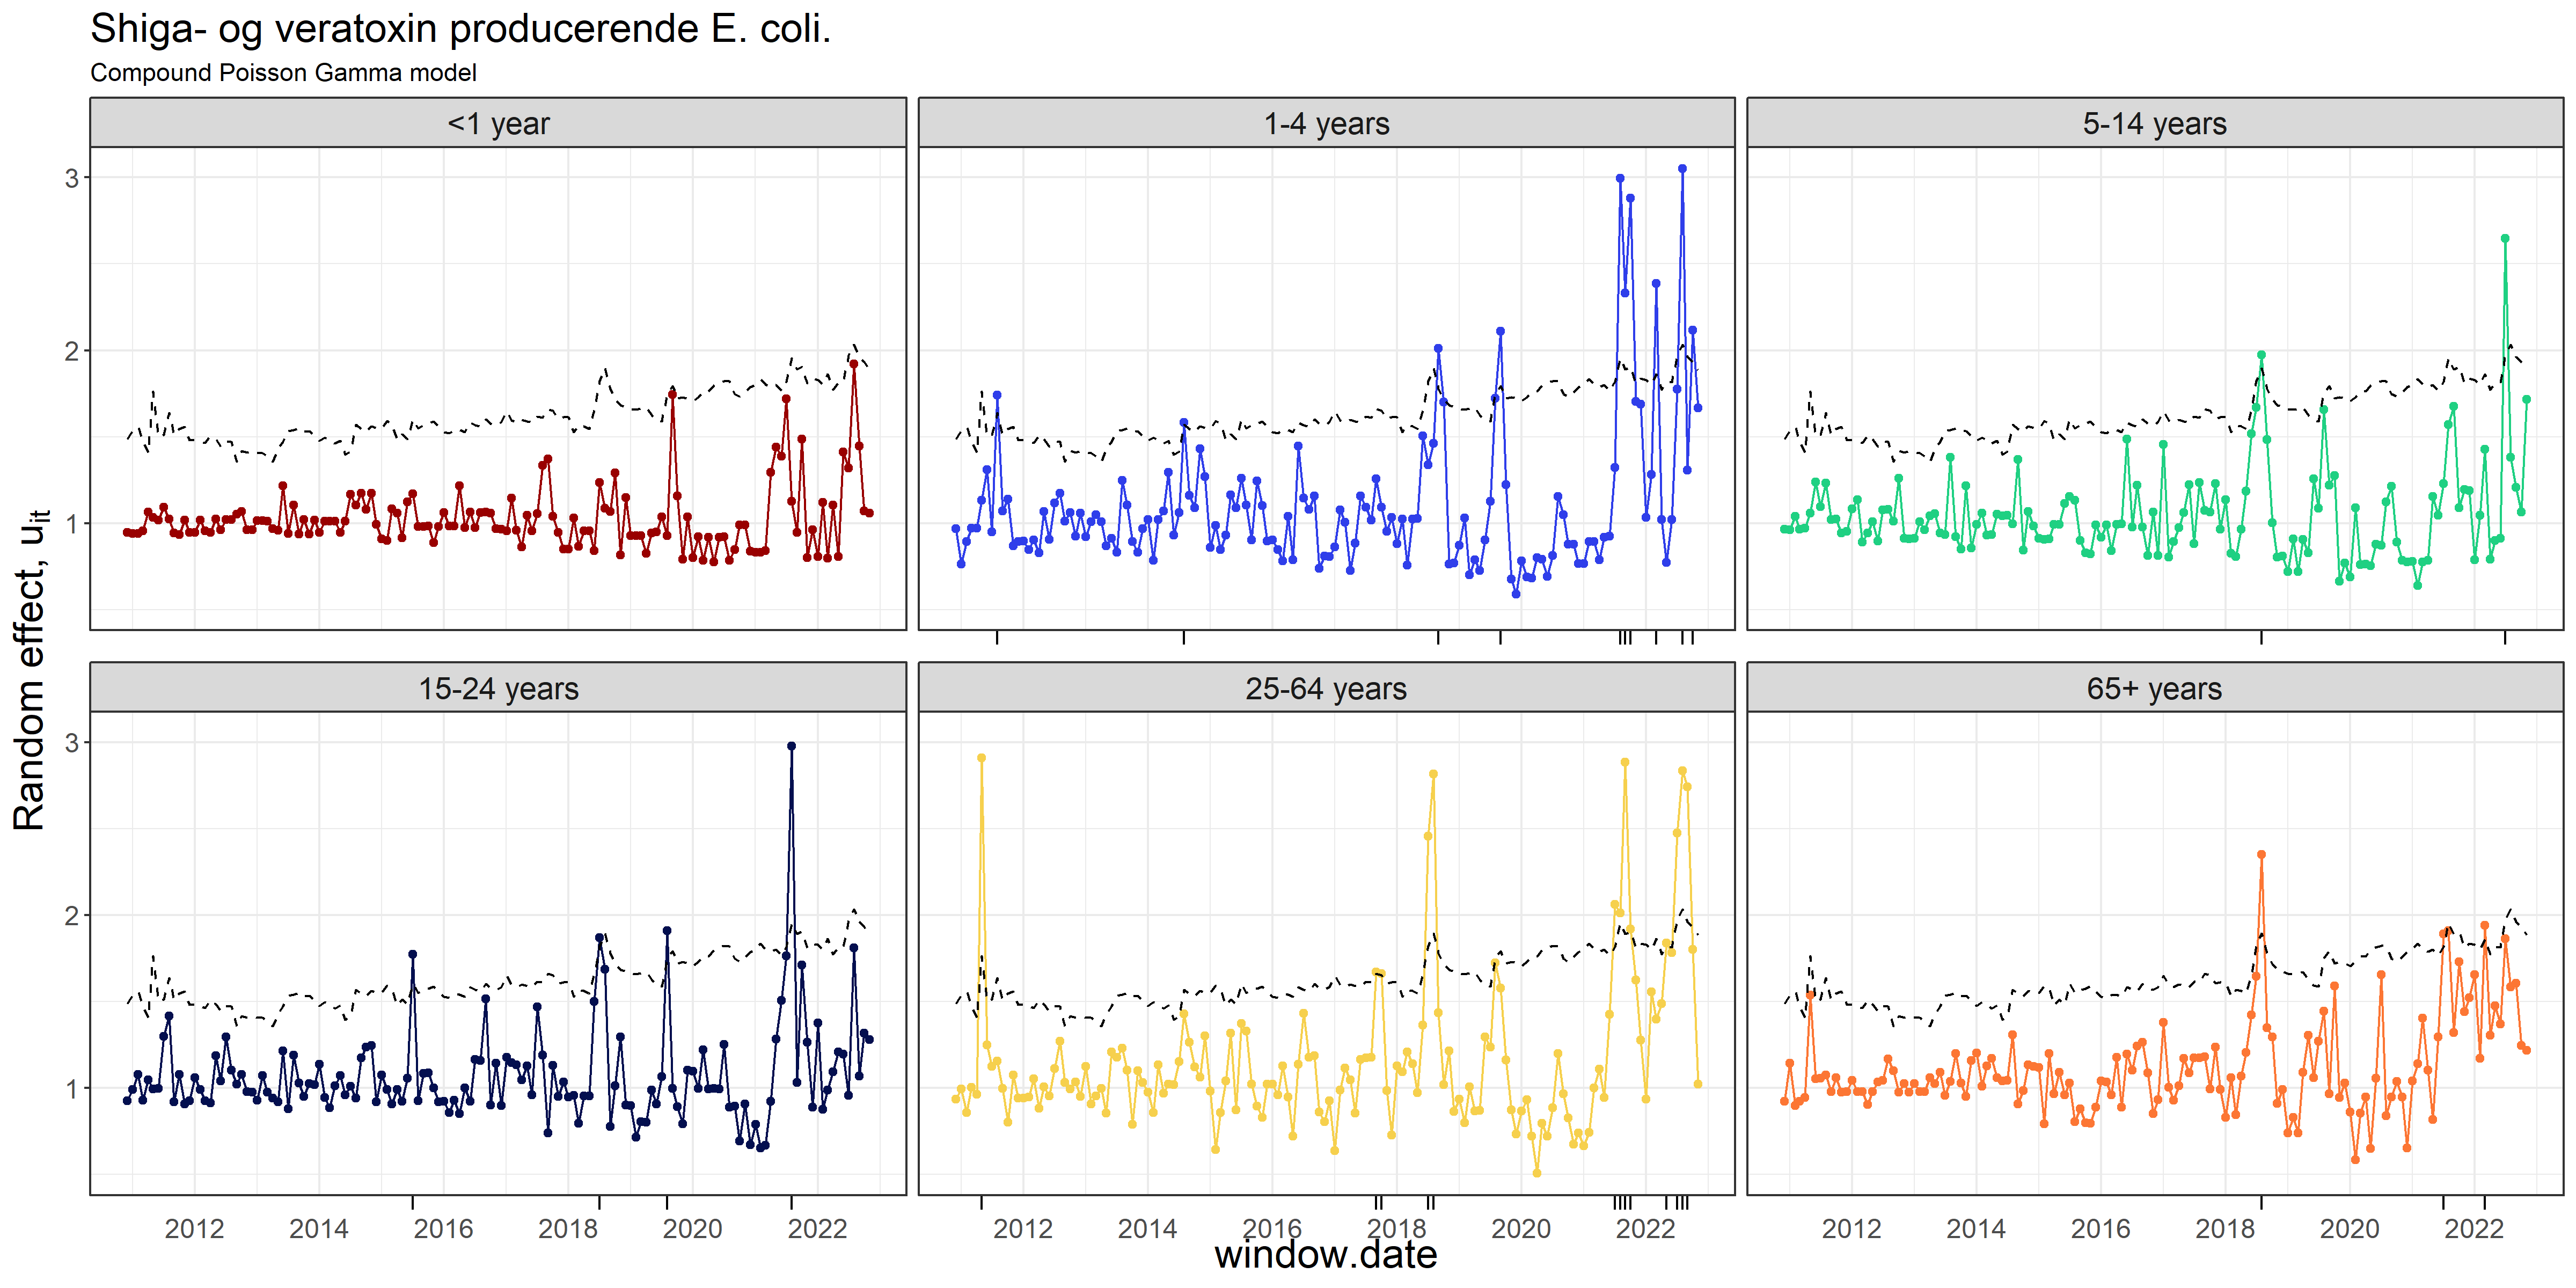
\includegraphics[width=1\linewidth]{../figures/windowedSTECPoisGExclude}

\normalsize
\end{frame}


\end{document}
